
\subsection{Spatial and time discretization}

The type of problems we will addressed in this project occur in a bounded
rectangular domain $\Omega \subset \real^2$, that is to say, there exist
non--degenerate intervals $I_X = [x_1, x_2]$ and $I_Y = [y_1, y_2]$ such that
$\Omega = I_X \times I_Y$. In order to solve the problem numerically we shall
follow a control--volume formulation is followed. This methodology discretizes
the domain into nonoverlapping control volumes along with a grid of points named
discretization nodes. The resulting discretized domain is named mesh or
numerical grid \cite{patankar2008numerical}.

There exist several types of grids according to the shape of control volumes and
the ammount of subdivisions the domain has been partitioned into, namely, a
structured (regular) grid, a block--structured grid and an unstructured grid
\cite{ferziger2002computational2grid}. However, henceforth we will only consider
structured regular grids. This formulation allows for two manners to discretize
the domain, namely, cell--centered and node--centered discretizations. The
former places discretization nodes over the domain and generates a
control--volume centered on each node. The latter first generates the
control--volumes, next places a node at the center of each one and finally sets
nodes at the border if necessary.

\begin{figure}[h]
	\centering
	\begin{subfigure}{.5\textwidth}
		\centering
		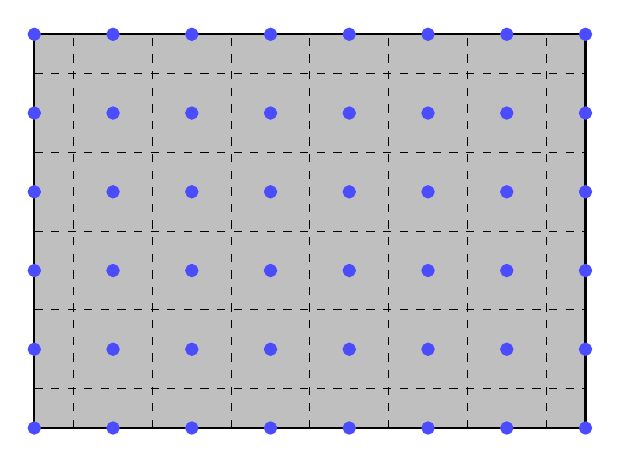
\begin{tikzpicture}
			\filldraw[black!50!white, opacity=0.5] (0,0) rectangle (7,5);
			\draw[black, thick] (0,0) rectangle (7,5);
			% Nodes
			\foreach \x in {0,1,...,7} {
				\foreach \y in {0,1,...,5} {
					\filldraw[blue!70!white, thick] (\x,\y) circle (2pt);
				}
			}
			% Control volumes
			\foreach \x in {0,1,...,6} {
				\draw[black, dashed] ({\x+0.5},0) -- ++(0,5);
			}
			\foreach \y in {0,1,...,4} {
				\draw[black, dashed] (0,{\y+0.5}) -- ++(7,0);
			}
		\end{tikzpicture}
		\caption{Cell--centered uniform discretization.}
		\label{fig:face_node_centered_discretization_comparison_1}
	\end{subfigure}%
	\begin{subfigure}{.5\textwidth}
		\centering
		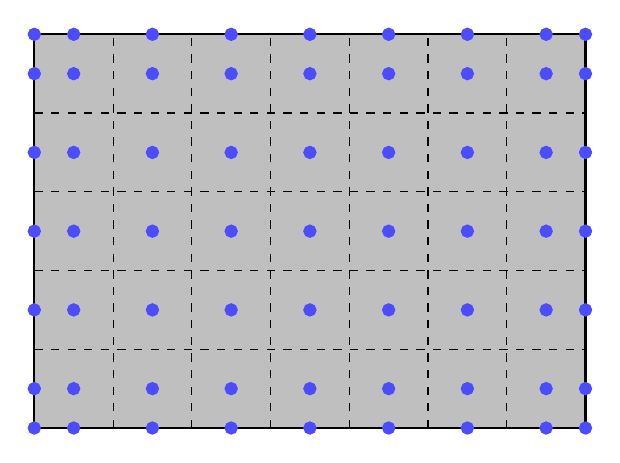
\begin{tikzpicture}
			\filldraw[black!50!white, opacity=0.5] (0,0) rectangle (7,5);
			\draw[black, thick] (0,0) rectangle (7,5);
			% Control volumes
			\foreach \x in {1,...,6} {
				\draw[black, dashed] (\x,0) -- ++(0,5);
			}
			\foreach \y in {1,...,4} {
				\draw[black, dashed] (0,\y) -- ++(7,0);
			}
			% Internal nodes
			\foreach \x in {0,1,...,6} {
				\foreach \y in {0,1,...,4} {
					\filldraw[blue!70!white, thick] ({\x+0.5},{\y+0.5}) circle (2pt);
				}
			}
			% Lower and upper rows nodes
			\foreach \x in {0,1,...,6} {
				\filldraw[blue!70!white, thick] ({\x+0.5},0) circle (2pt);
				\filldraw[blue!70!white, thick] ({\x+0.5},5) circle (2pt);
			}
			% Left and right columns nodes
			\foreach \y in {0,1,...,4} {
				\filldraw[blue!70!white, thick] (0,{\y+0.5}) circle (2pt);
				\filldraw[blue!70!white, thick] (7,{\y+0.5}) circle (2pt);
			}
			% Corner nodes
			\foreach \x in {0,1} {
				\foreach \y in {0,1} {
					\filldraw[blue!70!white, thick] ({7*\x},{5*\y}) circle (2pt);
				}
			}
		\end{tikzpicture}
		\caption{Node--centered uniform discretization.}
		\label{fig:face_node_centered_discretization_comparison_2}
	\end{subfigure}
	\caption{Comparison of the cell--centered and the node--centered uniform discretizations.}
	\label{fig:face_node_centered_discretization_comparison}
\end{figure}

\noindent
As it can be noticed when uniform discretizations are used, the node--centered
discretization approach offers higher resolution near the boundary of the
domain. Notwithstanding, it also generates singular nodes located at the corners
which need a special treatment, whilst the cell--centered does not. Furthermore,
the discretizations can be uniform, which implies that the distances between
adjacent internal nodes are kept constant along the domain, or non--uniform,
meaning the opposite.

In regards to time, the problems we consider last for finite time. Therefore the
time interval is $I = [0, T] \subset \real$ with $T > 0$ finite. The
discretization of $I$ is simply a partition of it, that is to say, a finite set
of points $P(I) = \{ t_0 = 0, t_1, \ldots, t_{m-1}, t_m = T \}$ with $t_{i+1} >
t_i$ for all $0 \leq i < m$. The time discretization is said to uniform whenever
there exists $\Delta t > 0$ such that $t_{i+1} - t_i = \Delta t$ for all $i$,
and non--uniform otherwise. We shall only consider uniform time discretizations,
nevertheless non--uniform discretizations might be convenient in problems
combining fast and low transient processes.